\documentclass[12pt]{article}

%%%%%%%%%%%%%%%%%%%%%%%%%%%%%%%%%%%%%%%%%%%%%%%%%%%%%%%%%%%%%%%%%%%%%%%%%%%%%%%%
%                           Package preset for homework
%%%%%%%%%%%%%%%%%%%%%%%%%%%%%%%%%%%%%%%%%%%%%%%%%%%%%%%%%%%%%%%%%%%%%%%%%%%%%%%%
% Miscellaneous
\usepackage[margin=1in]{geometry}
\usepackage[utf8]{inputenc}
\usepackage{indentfirst}
\usepackage{blindtext}
\usepackage{graphicx}
\usepackage{xr-hyper}
\usepackage{hyperref}
\usepackage{enumitem}
\usepackage{color}
\usepackage{float}
% Math
\usepackage{latexsym}
\usepackage{amsfonts}
\usepackage{amssymb}
\usepackage{amsmath}
\usepackage{commath}
\usepackage{amsthm}
\usepackage{bbold}
\usepackage{bm}
% Physics
\usepackage{physics}
\usepackage{siunitx}
% Code typesetting
\usepackage{listings}
% Citation
\usepackage[authoryear]{natbib}
\usepackage{appendix}
\usepackage[capitalize]{cleveref}
% Title & name
\title{Homework}
\author{Tien Vo}
\date{\today}


%%%%%%%%%%%%%%%%%%%%%%%%%%%%%%%%%%%%%%%%%%%%%%%%%%%%%%%%%%%%%%%%%%%%%%%%%%%%%%%%
%                   User-defined commands and environments
%%%%%%%%%%%%%%%%%%%%%%%%%%%%%%%%%%%%%%%%%%%%%%%%%%%%%%%%%%%%%%%%%%%%%%%%%%%%%%%%
%%% Misc
\sisetup{load-configurations=abbreviations}
\newcommand{\due}[1]{\date{Due: #1}}
\newcommand{\hint}{\textit{Hint}}
\let\oldt\t
\renewcommand{\t}[1]{\text{#1}}

%%% Bold sets & abbrv
\newcommand{\N}{\mathbb{N}}
\newcommand{\Z}{\mathbb{Z}}
\newcommand{\R}{\mathbb{R}}
\newcommand{\Q}{\mathbb{Q}}
\let\oldP\P
\renewcommand{\P}{\mathbb{P}}
\newcommand{\LL}{\mathcal{L}}
\newcommand{\FF}{\mathcal{F}}
\newcommand{\HH}{\mathcal{H}}
\newcommand{\NN}{\mathcal{N}}
\newcommand{\ZZ}{\mathcal{Z}}
\newcommand{\RN}[1]{\textup{\uppercase\expandafter{\romannumeral#1}}}
\newcommand{\ua}{\uparrow}
\newcommand{\da}{\downarrow}

%%% Unit vectors
\newcommand{\xhat}{\vb{\hat{x}}}
\newcommand{\yhat}{\vb{\hat{y}}}
\newcommand{\zhat}{\vb{\hat{z}}}
\newcommand{\nhat}{\vb{\hat{n}}}
\newcommand{\rhat}{\vb{\hat{r}}}
\newcommand{\phihat}{\bm{\hat{\phi}}}
\newcommand{\thetahat}{\bm{\hat{\theta}}}

%%% Other math stuff
\providecommand{\units}[1]{\,\ensuremath{\mathrm{#1}}\xspace}
% Set new style for problem
\newtheoremstyle{problemstyle}  % <name>
        {10pt}                   % <space above>
        {10pt}                   % <space below>
        {\normalfont}           % <body font>
        {}                      % <indent amount}
        {\bfseries\itshape}     % <theorem head font>
        {\normalfont\bfseries:} % <punctuation after theorem head>
        {.5em}                  % <space after theorem head>
        {}                      % <theorem head spec (can be left empty, 
                                % meaning `normal')>

% Set problem environment
\theoremstyle{problemstyle}
\newtheorem{problemenv}{Problem}[section]
\newenvironment{problem}[1]{%
  \renewcommand\theproblemenv{#1}%
  \problemenv
}{\endproblemenv}
% Set lemma environment
\newenvironment{lemma}[2][Lemma]{\begin{trivlist}
\item[\hskip \labelsep {\bfseries #1}\hskip \labelsep {\bfseries #2.}]}{\end{trivlist}}
% Set solution environment
\newenvironment{solution}{
    \begin{proof}[Solution]$ $\par\nobreak\ignorespaces
}{\end{proof}}
\numberwithin{equation}{problemenv}

%%% Page format
\setlength{\parindent}{0.5cm}
\setlength{\oddsidemargin}{0in}
\setlength{\textwidth}{6.5in}
\setlength{\textheight}{8.8in}
\setlength{\topmargin}{0in}
\setlength{\headheight}{18pt}

%%% Code environments
\definecolor{dkgreen}{rgb}{0,0.6,0}
\definecolor{gray}{rgb}{0.5,0.5,0.5}
\definecolor{mauve}{rgb}{0.58,0,0.82}
\lstset{frame=tb,
  language=Python,
  aboveskip=3mm,
  belowskip=3mm,
  showstringspaces=false,
  columns=flexible,
  basicstyle={\small\ttfamily},
  numbers=none,
  numberstyle=\tiny\color{gray},
  keywordstyle=\color{blue},
  commentstyle=\color{dkgreen},
  stringstyle=\color{mauve},
  breaklines=true,
  breakatwhitespace=true,
  tabsize=4
}
\lstset{
  language=Mathematica,
  numbers=left,
  numberstyle=\tiny\color{gray},
  numbersep=5pt,
  breaklines=true,
  captionpos={t},
  frame={lines},
  rulecolor=\color{black},
  framerule=0.5pt,
  columns=flexible,
  tabsize=2
}


\title{Homework 8: Phys 5210 (Fall 2021)}

\begin{document}
\maketitle
%%%%%%%%%%%%%%%%%%%%%%%%%%%%%%%%%%%%%%%%%%%%%%%%%%%%%%%%%%%%%%%%%%%%%%%%%%%%%%%%
\begin{problem}{1}
Ever since the 16th century, we know that Earth orbits the Sun and not the other
way around. However, we are modern scientists and understand that there's
nothing wrong with looking at cosmos from the point of view of the Earth
reference frame. In that reference frame the Sun rotates around the Earth,
making a full rotation in close to 24 hours. The Sun is massive and its distance
to the Earth is large, thus the centripetal force which makes it move this way
must be very large. Identify the force which makes the Sun move in this way and
show that it provides correct acceleration to the Sun in the reference frame
which rotates with the Earth. Take into account that the vector connecting Earth
with the Sun forms an angle $\theta<\pi /2$ with the Earth's angular velocity
$\bm\Omega$. Neglect Earth's orbiting the Sun and the Sun's movement relative to
the center of the galaxy. In other words, you can assume for the purpose of this
problem that both the Earth and the Sun are stationary in space relative to
distant galaxies, and that the Earth rotates about its axis with a constant
angular velocity.
\begin{solution}
The rotation of the Earth about its axis is
$\bm\Omega=\Omega\qty(\cos\theta\yhat+\sin\theta\zhat)$ where $T=2\pi
/\Omega\approx 24$\,\si{hr}. In the inertial frame, let the Earth be at the
origin and the Sun at $\vb{r}=r\yhat$ where $r=1$\,\si{AU}. Then the force on
the Sun seen by an observer on Earth is
\begin{equation}\label{p1:F}
    \vb{F}=-2M\bm\Omega\times\vb{v}-M\bm\Omega\times(\bm\Omega\times\vb{r}) 
    =M\bm\Omega\times\qty(\bm\Omega\times\vb{r})
\end{equation}
where we have written $\vb{v}=-\bm\Omega\times\vb{r}$. Also, by Newton's 2nd
law, $\vb{F}=M\vb{a}$. So the acceleration of the Sun in the non-inertial frame
rotating with the Earth is 
\begin{equation}
    \vb{a}=\bm\Omega\times\qty(\bm\Omega\times\vb{r}) 
    =\Omega\qty(\cos\theta\yhat+\sin\theta\zhat)\times\qty(-\Omega r\xhat)
    =\Omega^2r\sin\theta\qty(\cos\theta\zhat-\sin\theta\yhat)
\end{equation}
So the magnitude of this acceleration is
\begin{equation}
    a=\Omega^2r\sin\theta\approx726\,\si{ms\tothe{-2}}
\end{equation}
where $\theta=66.6^\circ$ from online sources. Note that this is also the 
centripetal acceleration if the Sun rotates around the Earth in circular orbit 
with radius $r_\bot=r\sin\theta$ and angular velocity $\Omega$. So the force
\eqref{p1:F} gives the correct acceleration of the Sun.
\end{solution}
\end{problem}
%%%%%%%%%%%%%%%%%%%%%%%%%%%%%%%%%%%%%%%%%%%%%%%%%%%%%%%%%%%%%%%%%%%%%%%%%%%%%%%%    
%%%%%%%%%%%%%%%%%%%%%%%%%%%%%%%%%%%%%%%%%%%%%%%%%%%%%%%%%%%%%%%%%%%%%%%%%%%%%%%%
\begin{problem}{2}
Solve for the motion of the Foucault's pendulum. It is a pendulum attached to a
very high ceiling of a building located at a latitude $\phi$, swinging back and
forth along the floor with frequency $\omega$. For the purpose of calculating
its kinetic energy, neglect the vertical motion of the pendulum, taking its
movement as two dimensional. How long does it take for the plane of oscillations
to do one full rotation?
\begin{solution}
\begin{center}
    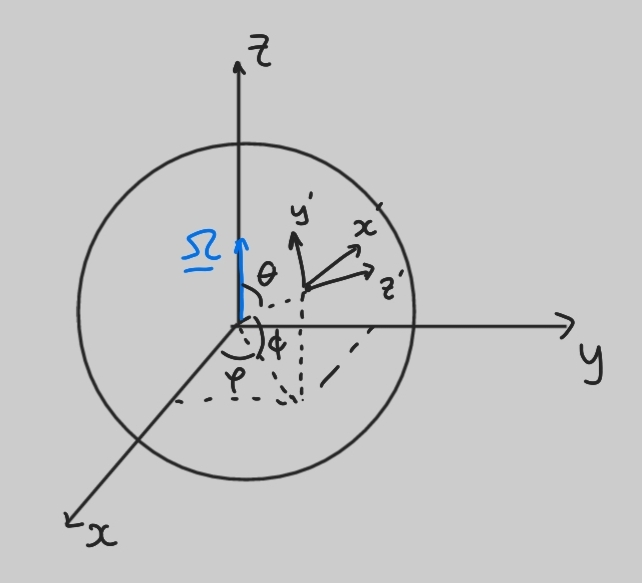
\includegraphics[width=0.5\textwidth]{hw8_p2.jpg} 
\end{center}
Define a coordinate system as above where $\rhat=\zhat',\thetahat=\yhat'$, and
$\phihat=\xhat'$. Then the Earth's rotation is
$\bm\Omega=\Omega(\cos\theta\zhat'-\sin\theta\yhat')$. The velocity of the
pendulum on the surface of the Earth at $\theta=\pi /2-\phi$, neglecting the
$\zhat'$ direction, is $\vb{v}'=\dot{\vb{x}}'=\dot{x}'\xhat'+\dot{y}'\yhat'$. 
Now, the force on a pendulum with frequency $\omega$ in the non-inertial 
reference frame of the Earth is
\begin{align}
    &&\vb{F}&=m\vb{a}'=-m\omega^2\vb{x}'-2m\bm\Omega\times\vb{v}'\notag\\
    &\Rightarrow&\vb{a}'
    &=-\omega^2\vb{x}'-2\Omega\qty(\cos\theta\zhat'-\sin\theta\yhat')
    \times\qty(\dot{x}'\xhat'+\dot{y}'\yhat')\notag\\
    &\Leftrightarrow&\vb{a}'
    &=-\omega^2\vb{x}'-2\Omega\cos\theta\qty(\dot{x}'\yhat'-\dot{y}'\xhat')
\end{align}
where the $\zhat'$ component is ignored. Writing $\cos\theta=\sin\phi$, we then
have the following system of differential equations
\begin{subequations}
    \begin{align}
        \ddot{x}&=-\omega^2x+2\Omega\sin\phi\dot{y}\\ 
        \ddot{y}&=-\omega^2y-2\Omega\sin\phi\dot{x}
    \end{align} 
\end{subequations}
where we have dropped the primes to simplify the expressions. Letting $z=x+iy$,
then the system above can be simplified into a single differential equation
\begin{equation}
    \ddot{z}=\ddot{x}+i\ddot{y}
    =-\omega^2(x+iy)-2i\Omega\sin\phi(\dot{x}+i\dot{y})
    \Rightarrow
    \ddot{z}+\omega^2z+2i\Omega\sin\phi\dot{z}=0
\end{equation}
Solving this with Mathematica yields the solution
\begin{equation}\label{p2:z}
    z(t)=e^{-i\Omega\sin\phi
    t}\qty[A\sin\qty(\sqrt{\omega^2+\Omega^2\sin^2\phi}t)
    +B\cos\qty(\sqrt{\omega^2+\Omega^2\sin^2\phi}t)] 
\end{equation}
where $A,B$ are constants dependent on initial conditions. We can also write
explicitly
\begin{subequations}
    \begin{align}
        x(t)&=\Re\qty{z}
        =\cos(\Omega\sin\phi t)\qty[A\sin\qty(\sqrt{\omega^2+\Omega^2\sin^2\phi}t)
    +B\cos\qty(\sqrt{\omega^2+\Omega^2\sin^2\phi}t)]\\
        y(t)&=\Im\qty{z}
        =-\sin(\Omega\sin\phi t)\qty[A\sin\qty(\sqrt{\omega^2+\Omega^2\sin^2\phi}t)
    +B\cos\qty(\sqrt{\omega^2+\Omega^2\sin^2\phi}t)] 
    \end{align} 
\end{subequations}
However, from \eqref{p2:z}, it is more apparent that the amplitude of
the sinuisoidal solution (in the square bracket) is rotated in the $x'y'$ plane 
clockwise with a frequency $\Omega\sin\phi$. Thus, the time it takes for the 
plane of oscillations to do one full rotation is
\begin{equation}
    T=\frac{2\pi}{\Omega\sin\phi} 
\end{equation}
\end{solution}
\end{problem}
%%%%%%%%%%%%%%%%%%%%%%%%%%%%%%%%%%%%%%%%%%%%%%%%%%%%%%%%%%%%%%%%%%%%%%%%%%%%%%%%
\end{document}
